%calcul de l'age
\newcounter{dateone}%
\newcounter{datetwo}%
\setmydatenumber{dateone}{1982}{05}{23}%
\setmydatenumber{datetwo}{\the\year}{\the\month}{\the\day}%
\FPsub\result{\thedatetwo}{\thedateone}
\FPdiv\myage{\result}{365.2425}

\begin{frame}{Mathieu Leocmach, {\normalsize\FPtrunc\myage{\myage}{0}\myage ~ans}\hfill \hspace{4.7cm}Cursus}
%photo
\newlength{\totorowidth}%
\newsavebox{\totorobox}%
\savebox\totorobox{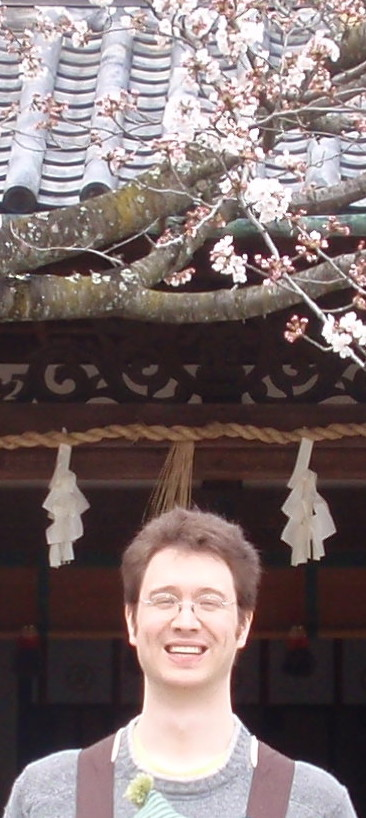
\includegraphics[height=\textheight-\headheight-\footheight-2em]{shikoku.jpg}}%
\settowidth{\totorowidth}{\usebox{\totorobox}}%
%
\begin{columns}[b]
\column{0.7\textwidth}
\begin{description}[2002-05]
\item[2002-05] \nth{1} Master \hfill{\footnotesize Ecole Polytechnique}
\item[2006-08] \nth{2} Master \hfill{\footnotesize Univ. Tokyo}
\item[2008-11] PhD \hfill{\footnotesize Univ. Tokyo}
\item[2011-12] Postdoc \hfill{\footnotesize Univ. Tokyo}
\item[2012-\hfill] Postdoc \hfill{\footnotesize E.N.S. de Lyon}\\
{\footnotesize $\approx$ 60 h/year teaching: 
\begin{itemize}
\item Physics long ($6\times \SI{8}{\hour}$) lab work (Master)
\item Python programming (L3)
\end{itemize}}
\end{description}


\begin{block}{9 articles (5 as first author)\\
\footnotesize 10 invited talks, 4 contributed, 18 posters}
\footnotesize 
\begin{description}[Crystal]
\item[Glass] Nature Commun., J. Chem. Phys., AIP Conf. Proc.
\item[Crystal] Soft Matter, Europhys. Lett.
\item[Oscil. reaction] Chemical Communications
\item[Gel] Phys. Rev. Lett., Macromol. Rapid Commun.
\item[Teaching] Bulletin de l'Union des Physiciens
\hfill\raisebox{0.6\normalbaselineskip}[0pt][0pt]{$\left.\rule{0pt}{1.2\normalbaselineskip}\right\}$ 2014}
\end{description}
\end{block}
\column{\totorowidth}
\usebox{\totorobox}
\end{columns}
\end{frame}

\begin{frame}{PhD: colloidal glass transition}

\begin{block}{Dynamic heterogeneity, candidate structural causes}
\begin{columns}
\column{0.25\textwidth}
\tikzsetnextfilename{dh_perera}\begin{tikzpicture}
\node[inner sep=0] (dh) {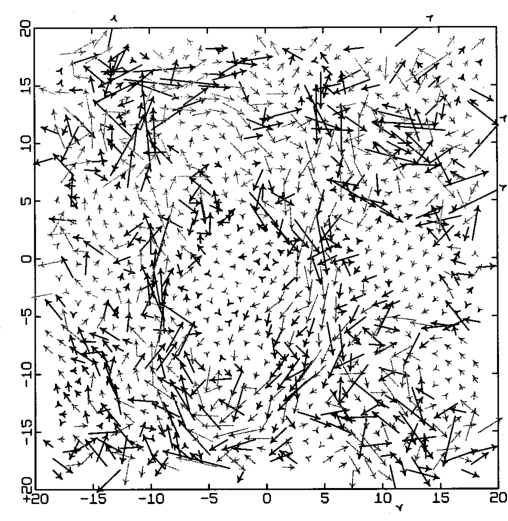
\includegraphics[width=\textwidth]{dh_perera}};
\node[below=0 of dh.north, inner sep=1pt, fill=white, font=\footnotesize\itshape] {Perera 1999};
\end{tikzpicture}
\column{0.6\textwidth}
\begin{enumerate}
\item locally stable structures\\
\tikzsetnextfilename{pentagons}\begin{tikzpicture}[pen/.style={regular polygon, regular polygon sides=5, draw, minimum size=0.4\baselineskip}]
	\node[pen] (base) {};
	\node[pen,anchor=south, rotate=180] at (base.side 3) {};
	\node[pen,anchor=south, rotate=-108] at (base.side 4) {};
\end{tikzpicture}
\hfill {\footnotesize icosahedra}
\item avoided crystal influence\\
\newdimen\radius
\setlength{\radius}{0.3\baselineskip}
\tikzsetnextfilename{localangles}\begin{tikzpicture}
	\begin{scope}[rotate=80, every node/.style={circle, fill, color=Accent1!50, inner sep=0, minimum size=1.8\radius}]
		%first neighbourhood
		\fill node (a) {} +(30:2.1\radius) node (b) {} +(90:2.2\radius) node (c) {} +(150:2.05\radius) node (d) {} +(210:2.3\radius) node (e) {} +(270:2.2\radius) node (f) {} +(330:2.01\radius) node (g) {};
		%second neighbourhood
		\fill ++(g) ++(-70:2.01\radius) node (h) {} +(40:2.01\radius) node (i) {} +(220:2.2\radius) node (j) {} +(280:2.05\radius) node (k) {} +(340:2.05\radius) node (l) {};
		\fill ++(j) ++(-70:2.2\radius) node (m) {} +(170:2.01\radius) node (n) {} +(230:2.2\radius) node (o) {} +(290:2.05\radius) node (p) {} +(350:2.05\radius) node (q) {};
	\end{scope}
	\coordinate (corner) at (e.west|-p.south);
	\tikzset{ar/.style={->, draw=Main, thick}}
	\draw[ar] (d.center) -- (a.center);
	\draw[ar] (f.center) -- (h.center);
	\draw[ar] (n.center) -- (m.center);
	\begin{scope}[green!50!black]
		\draw (c.center) -- (a.center) -- (b.center) (o.center) -- (m.center) -- (p.center);
		\path[<->] (c.center) edge [bend left] (b.center);
		\path[<->] (p.center) edge [bend left] (o.center);
	\end{scope}
\end{tikzpicture}
\hfill \textsc{\footnotesize fcc}
\end{enumerate}
\column{0.12\textwidth}
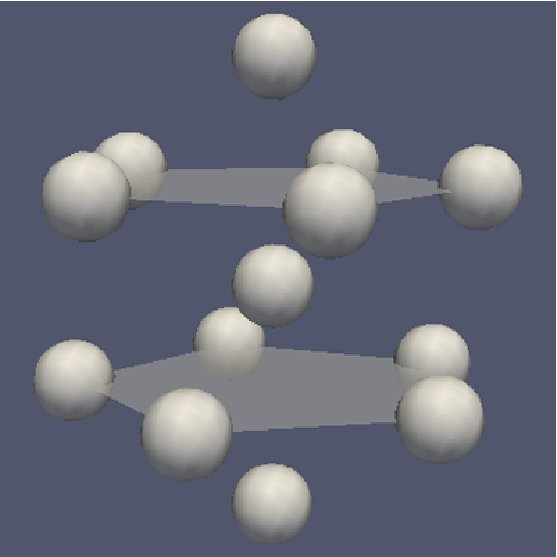
\includegraphics[width=\textwidth]{ico_13}\\
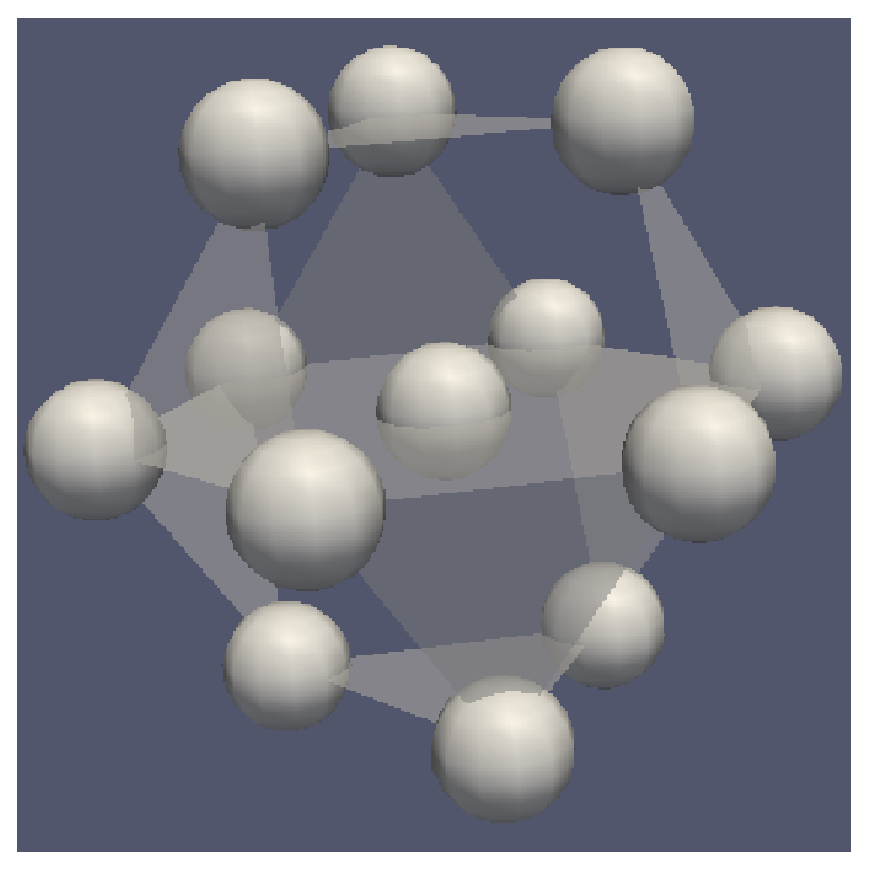
\includegraphics[width=\textwidth]{fcc_13}
\end{columns}
\end{block}
\structure{Single-particle colloidal experiments}

\smallskip
\tikzsetnextfilename{ico_dyn}\begin{tikzpicture}
	\begin{groupplot}[%
		group style = {
			group name=g,
			group size=2 by 1,
			horizontal sep = 3em
		},
		height=10em,%Tout est controlle par cette longueur
		width=0.35\columnwidth,
		label shift=-0.5em, %
		]
	\nextgroupplot[
		cycle list name=black white,
		every mark/.append style={scale=1.2},
		xlabel=$\phi$, xmin=0.49, xmax=0.58, xlabel near ticks,%
		xtick={0.5,0.53,...,0.6},%
		ylabel=$\xi/\xi_0$, ymax=10,
		ytick={2,4,6,8},
		legend pos=north west,%
		]
		\addplot+[only marks, mark=*, %
			every mark/.append style={fill=black, scale=1.2},
			error bars/.cd, y dir=both, y explicit relative,%
			] table[x index=0, y expr=\thisrowno{3}/0.126]{scale.xi};
		\addplot+[mark=none, forget plot, domain=0.49:0.58] {(0.6/x-1)^(-2.0/3.0)};
		\addplot+[only marks, mark=square, every mark/.append style={draw=gray, scale=1.2},] table[x index=0, y expr=\thisrowno{5}/0.216]{scale.xi};
		\legend{dynamic, crystalline};
	\nextgroupplot[
		ylabel={$\xi/\sigma$},
		ymax=1.9,
		xlabel={Pressure},
		ymin=0,
		xmin=8,
		xtick={9,13,...,25},]
	\pgfplotstableread{lengths}\lengths
	\addplot+[Main,every mark/.append style={fill=Main}] table[x index=0, y index=5]{\lengths} node[above left] {crystalline};
	\addplot+[Accent2,every mark/.append style={fill=Accent2}] table[x index=0, y index=4]{\lengths} node[above left] {icosahedral};
\end{groupplot}
%
\newdimen\mydima
\newdimen\mydimb
\pgfextracty{\mydima}{\pgfpointanchor{g c1r1}{north}}
\pgfextracty{\mydimb}{\pgfpointanchor{g c1r1}{south}}
\pgfmathsetlength{\mydima}{\mydima-\mydimb}
%
\begin{scope}[inner sep=0]
\node[anchor= south west] (mrco) at ($(g c2r1.right of south east)+(-\textwidth,0)$) {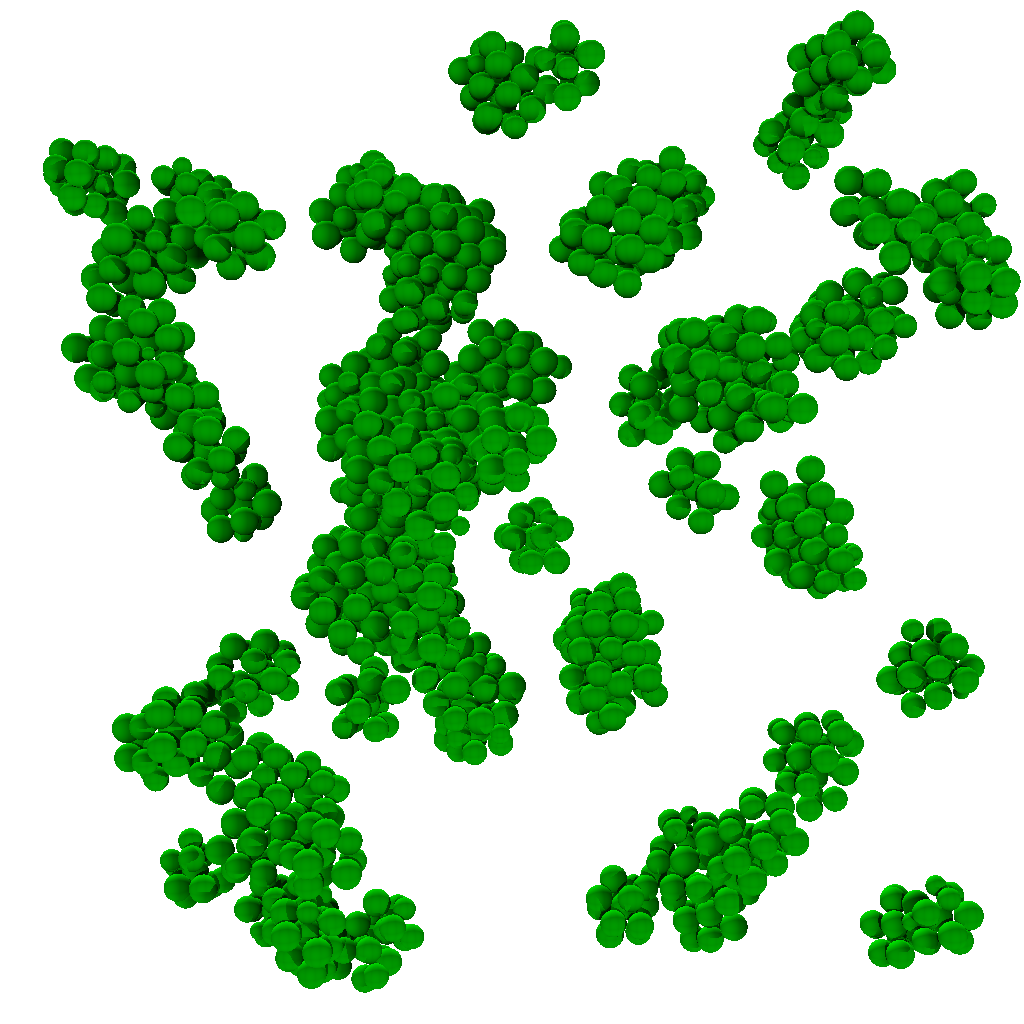
\includegraphics[height=\mydima]{mrco24_scale_go1_t040_t048.png}};
\node [below right=0 and 0.01\textwidth of mrco.north east] (slow) {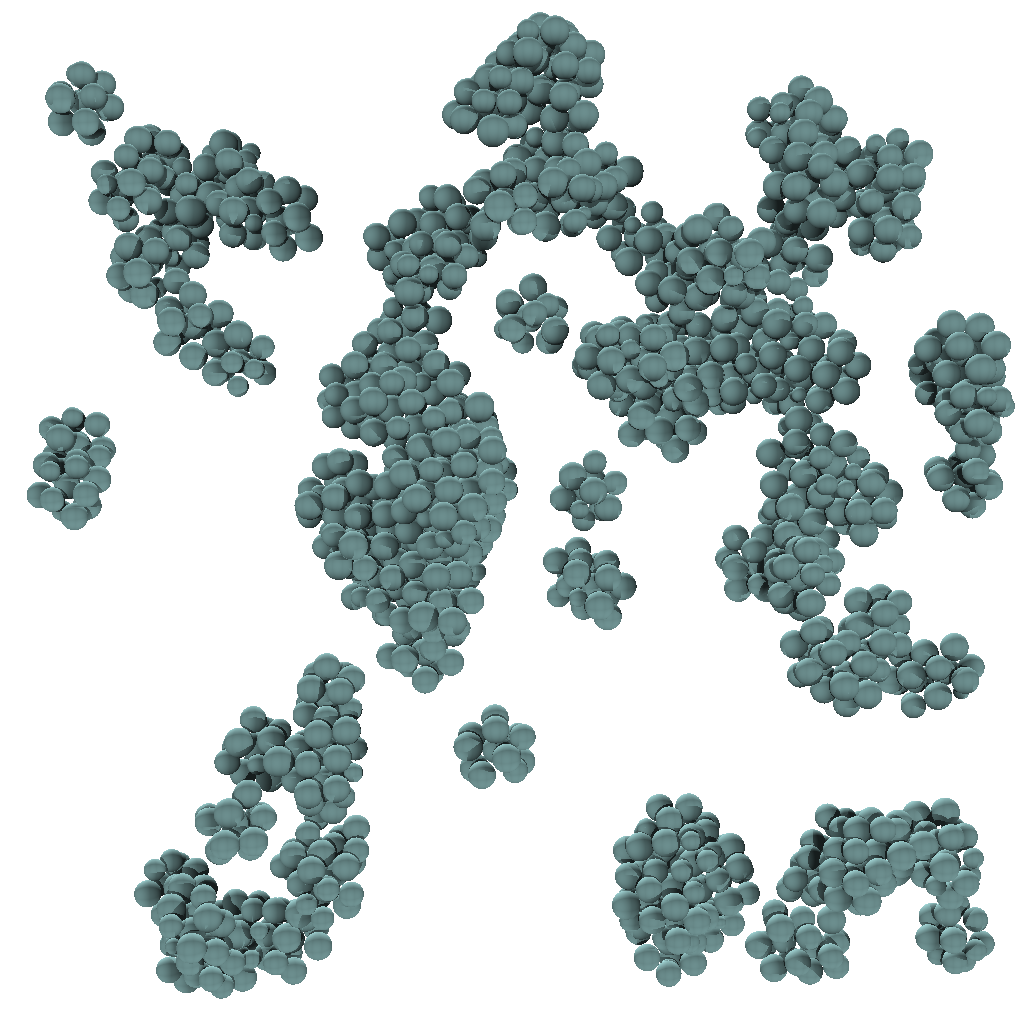
\includegraphics[height=\mydima]{cgsd_2tau.png}};
%labels
\begin{scope}[align=center]
	\node[below=0.2em of mrco, text width=\mydima] {crystal-like};
	\node[below=0.2em of slow, text width=\mydima]  {slow};
\end{scope}
\draw [help lines, step=0.25\mydima, shift=(mrco.south west)] (0, 0) grid (\mydima, \mydima);
	\draw [help lines, step=0.25\mydima, shift=(slow.south west)] (0, 0) grid (\mydima, \mydima);
\end{scope}
%\node[inner sep=0, draw, fit=(mrco) (g c2r1.outer south east) (g c1r1.outer south)]{};
\end{tikzpicture}
\begin{scriptsize}
Experiments \myfullcite{Leocmach2012}

Simulations \myfullcite{Leocmach2013a}
\end{scriptsize}

\end{frame}


%\begin{frame}{Des colloïdes pour comprendre les solidifications}
%\begin{columns}[onlytextwidth,b]
%\column{0.7\textwidth}
%\begin{block}{Les colloïdes comme modèles d'atomes}
%\textit{\footnotesize Einstein 1905, Perrin 1913}
%\begin{itemize}
%\item gros
%\item lents 
%	\raisebox{0.6\normalbaselineskip}[0pt][0pt]{$\left.\rule{0pt}{1.1\normalbaselineskip}\right\}$ visibles (confocal)}
%\item synthèses, solvants $\rightarrow$ interactions
%\hfill\tikzsetnextfilename{schema_interactions}\raisebox{0pt}[0pt][0pt]{\begin{tikzpicture}[scale=1.25]
%\input{fig_presentation/schema_interactions.pgf}
%\end{tikzpicture}}
%\end{itemize}
%\end{block}
%%
%\column{0.25\textwidth}
%Image confocale\\
%\includegraphics[width=\textwidth]{draft_nwk_dense_perco.jpg}
%\end{columns}
%%
%\structure{Accès aux coordonnées et trajectoires}\\
%Analyses de données détaillées sur le système réel avec toute sa richesse physico-chimique
%\end{frame}
%
%\begin{frame}{PhD : Transition vitreuse}
%\begin{columns}
%	\column{0.5\textwidth}
%	\tikzsetnextfilename{glass_cooling}\begin{tikzpicture}
\newdimen\mrad
\setlength{\mrad}{0.75em}
\begin{axis}[
	name=glass,
	width=\textwidth, height=0.75\textwidth,
	xlabel=Temperature, xmin=0, xmax=1.25, axis x line=bottom, xtick=\empty,%
	extra x ticks={0.2, 0.45, 0.7, 0.95}, extra x tick labels={$T_0$, $T_G$,,$T_m$},%
	xlabel shift=-0.5em,
	ylabel=Entropy, ymin=0.1, ymax=1.2, axis y line=left, ytick=\empty, ylabel shift=-0.5em,%
	axis on top,
	]
		\fill[gray!20] (axis cs:0.45, 0.45) .. controls (axis cs:0.325, 0.325) .. (axis cs:0,0.3) -- (axis cs:0, 0.18) -- (axis cs:0.45, 0.227) -- cycle;
		\draw (axis cs:0, 0.18) -- (axis cs:0.95, 0.28);
		\coordinate (Tt) at (axis cs:1.2,1.2);
		\coordinate (O) at (axis cs:0,0);
		\path[
			every node/.style={circle, inner sep=0.15em, outer sep=0, fill=magenta},
			every label/.style={rectangle, fill=none, anchor=south east, inner sep=0.1em, font=\tiny},
			label position=above left, 
			] (axis cs:0.2, 0.2)-- (Tt) 
			node[pos=0, label=$\tau\rightarrow\infty$ ?](T0){} 
			node[pos=0.25, label=$\tau\sim10^{3}$ s](Tg){} 
			node[pos=0.5, label=$\tau\sim10^{-9}$ s](Tc){} 
			node[pos=0.75, label=$\tau\sim10^{-13}$ s](Tm){};
		\draw (Tg) -- (Tt);
		\begin{scope}[decoration={text along path,transform={yshift=-0.9em}}]
			\draw[decorate, decoration={text={|\itshape\footnotesize|liquid}}] (Tm)--(Tt);
			\draw[decorate, decoration={text={|\itshape\footnotesize|supercooled},text align={align=center}}] (Tg)--(Tm);
		\end{scope}
		\draw[dotted] (T0)-- (Tg);
		\draw[help lines] (T0) -- (T0|-O) (Tg) -- (Tg|-O) (Tc) -- (Tc|-O) (Tm) -- (Tm|-O);

		\draw[red] (Tg) .. controls (axis cs:0.375, 0.375) .. (axis cs:0,0.35) node[pos=0.85, above, black,font=\itshape\footnotesize] {glass};
		\draw[orange] (Tg) .. controls (axis cs:0.35, 0.35) .. (axis cs:0,0.325);
		\draw[yellow] (Tg) .. controls (axis cs:0.325, 0.325) .. (axis cs:0,0.3);
\end{axis}

%\draw (glass.outer north west) rectangle +(\textwidth,-\textheight);
\end{tikzpicture}
%	%\begin{footnotesize}\citet{cavagna2009supercooled}\end{footnotesize}
%\column{0.5\textwidth}
%	\begin{itemize}
%		\item Refroidir un liquide
%		\item Cristallisation évitée
%		\item Temps de relaxation $\times 10^{10+}$
%		\item Sous $T_g$ solide non cristallin
%		\item Impossible d'approcher la divergence
%		\item Problème ouvert
%	\end{itemize}
%\end{columns}
%\begin{block}{Hétérogénéités dynamiques, causes structurelles proposées}
%\begin{columns}
%\column{0.25\textwidth}
%\tikzsetnextfilename{dh_perera}\begin{tikzpicture}
%\node[inner sep=0] (dh) {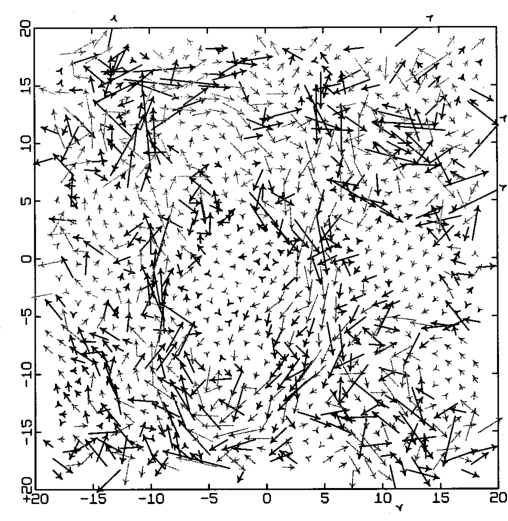
\includegraphics[width=\textwidth]{dh_perera}};
%\node[below=0 of dh.north, inner sep=1pt, fill=white, font=\footnotesize\itshape] {Perera 1999};
%\end{tikzpicture}
%\column{0.6\textwidth}
%\begin{enumerate}
%\item structures localement stables\\
%\tikzsetnextfilename{pentagons}\begin{tikzpicture}[pen/.style={regular polygon, regular polygon sides=5, draw, minimum size=0.4\baselineskip}]
%	\node[pen] (base) {};
%	\node[pen,anchor=south, rotate=180] at (base.side 3) {};
%	\node[pen,anchor=south, rotate=-108] at (base.side 4) {};
%\end{tikzpicture}
%\hfill {\footnotesize icosaèdre}
%\item influence du cristal évité\\
%\newdimen\radius
%\setlength{\radius}{0.3\baselineskip}
%\tikzsetnextfilename{localangles}
%\hfill \textsc{\footnotesize fcc}
%\end{enumerate}
%\column{0.12\textwidth}
%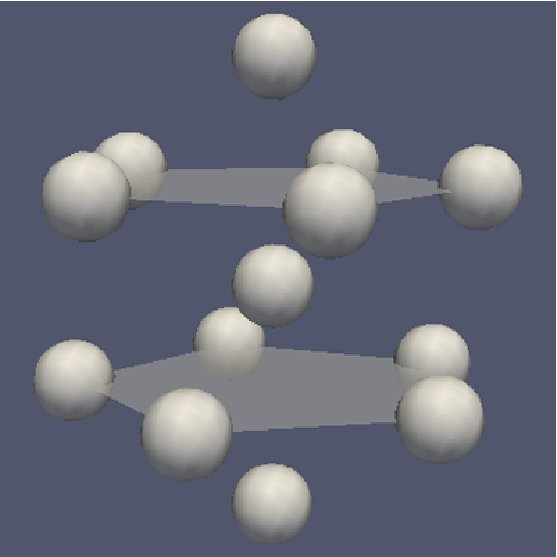
\includegraphics[width=\textwidth]{ico_13}\\
%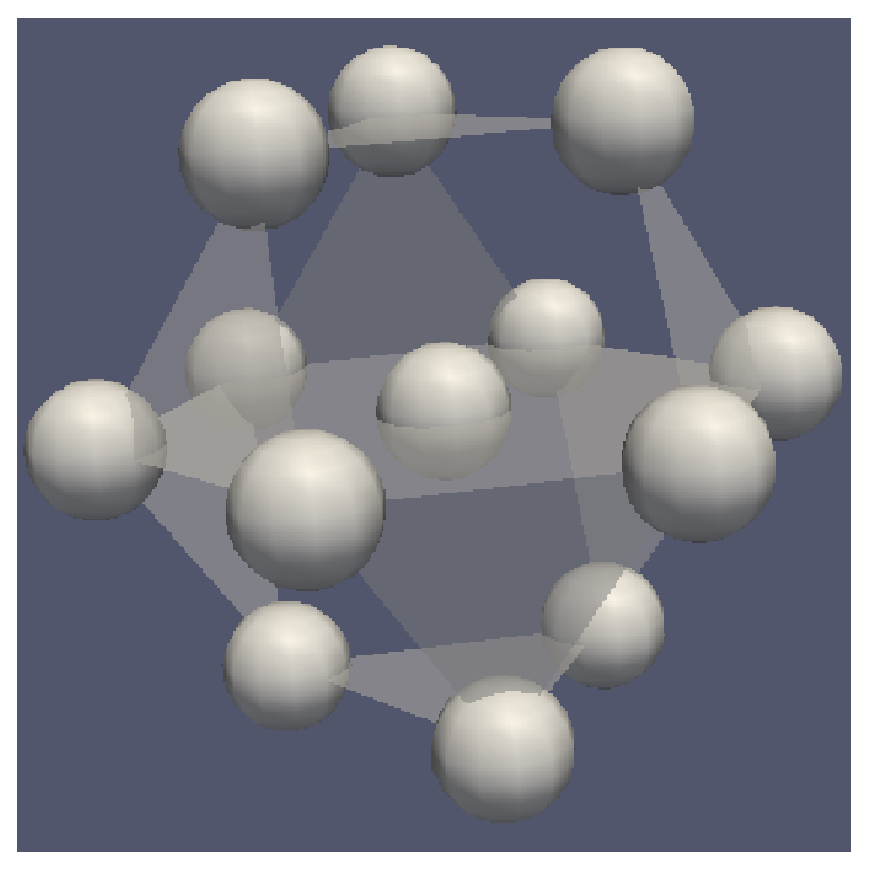
\includegraphics[width=\textwidth]{fcc_13}
%\end{columns}
%\end{block}
%\end{frame}
%
%\begin{frame}{PhD : Le cristal évité gouverne la dynamique}
%
%\begin{columns}
%\column{0.55\textwidth}
%\tikzsetnextfilename{mrco_slow}\begin{tikzpicture}[inner sep=0]
%\node (mrco) {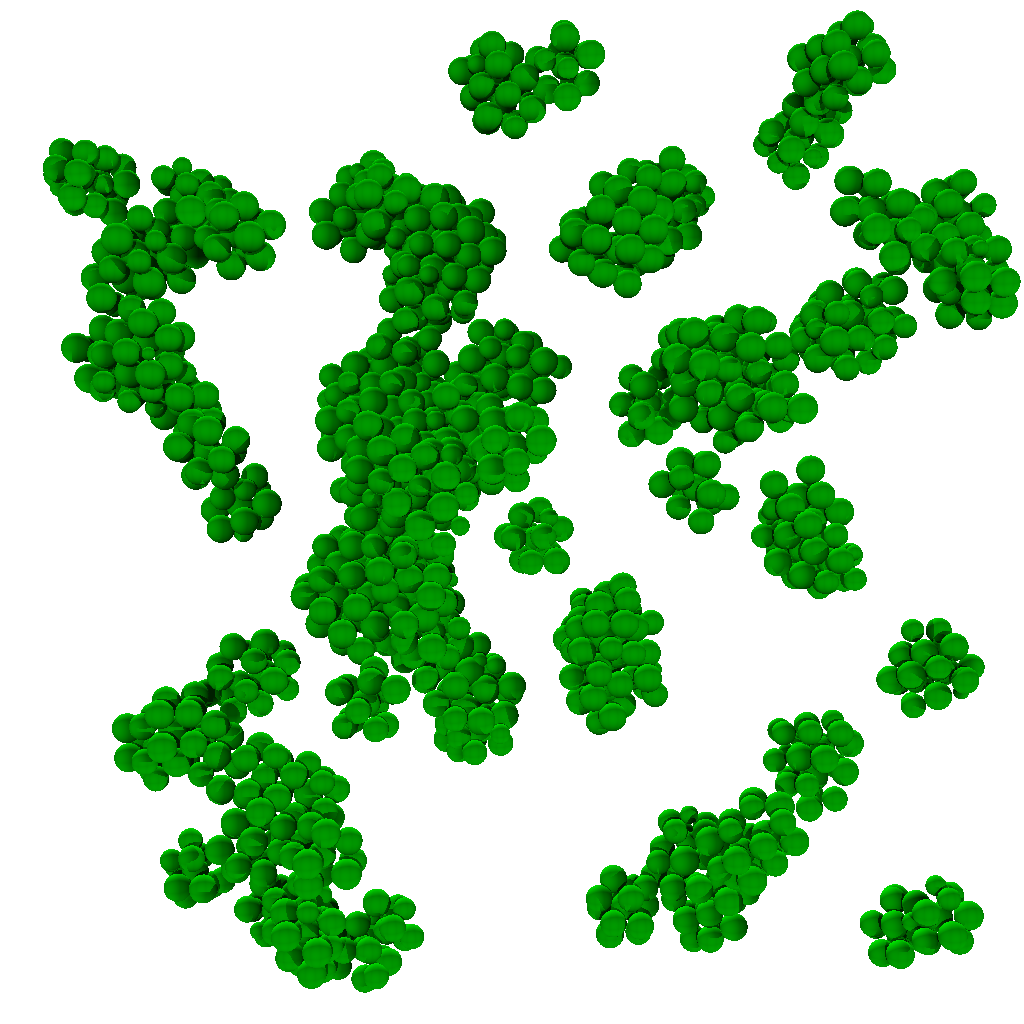
\includegraphics[height=0.48\textwidth]{mrco24_scale_go1_t040_t048.png}};
%\node [below right=0 and 0.04\textwidth of mrco.north east] (slow) {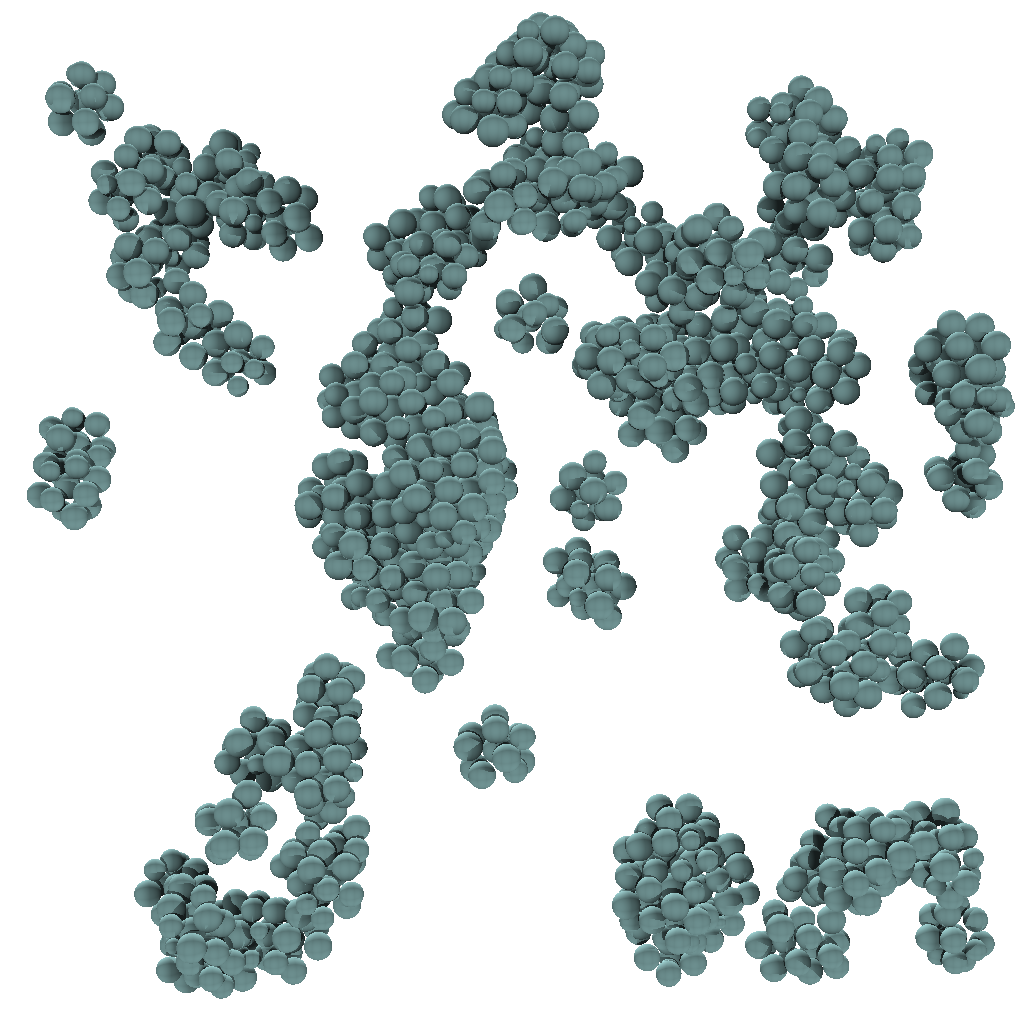
\includegraphics[height=0.48\textwidth]{cgsd_2tau.png}};
%%labels
%\begin{scope}[align=center, every node/.style={font=\footnotesize}]
%	\node[above=0of mrco, text width=0.48\textwidth] {ordre proto-cristallin};
%	\node[above=0of slow, text width=0.48\textwidth]  {particules lentes};
%\end{scope}
%\draw [help lines, step=0.12\textwidth, shift=(mrco.south west)] (0, 0) grid (0.48\textwidth, 0.48\textwidth);
%	\draw [help lines, step=0.12\textwidth, shift=(slow.south west)] (0, 0) grid (0.48\textwidth, 0.48\textwidth);
%\end{tikzpicture}
%\end{columns}
%%\[ \xi(\phi) \propto \xi_0 \left( \frac{\phi_0 - \phi}{\phi} \right)^{-\frac{2}{3}} \]
%
%
%\smallskip
%\structure{Longueurs de corrélation}\\
%\tikzsetnextfilename{corelation_lengths}\begin{tikzpicture}
%	\begin{groupplot}[%
%		group style = {
%			group size=2 by 1,
%			horizontal sep = 4em
%		},
%		height=0.34\columnwidth,%
%		width=0.5\columnwidth,
%		label shift=-0.5em, %
%		]
%	\nextgroupplot[
%		cycle list name=black white,
%		every mark/.append style={scale=1.2},
%		xlabel=$\phi$, xmin=0.49, xmax=0.58, xlabel near ticks,%
%		xtick={0.5,0.52,...,0.6},%
%		ylabel=$\xi/\xi_0$, ymax=10,
%		ytick={2,4,6,8},
%		legend pos=north west,%
%		]
%		\addplot+[only marks, mark=*, %
%			every mark/.append style={fill=black, scale=1.2},
%			error bars/.cd, y dir=both, y explicit relative,%
%			] table[x index=0, y expr=\thisrowno{3}/0.126]{scale.xi};
%		\addplot+[mark=none, forget plot, domain=0.49:0.58] {(0.6/x-1)^(-2.0/3.0)};
%		\addplot+[only marks, mark=square, every mark/.append style={draw=gray, scale=1.2},] table[x index=0, y expr=\thisrowno{5}/0.216]{scale.xi};
%		\legend{dynamique, cristalline};
%	\nextgroupplot[
%		ylabel={$\xi/\sigma$},
%		ymax=2,
%		xlabel={Pression},
%		ymin=0,
%		xmin=8,
%		xtick={9,13,...,25},]
%	\pgfplotstableread{lengths}\lengths
%	\addplot+[Main] table[x index=0, y index=5]{\lengths} node[above left] {cristal};
%	\addplot+[Accent2] table[x index=0, y index=4]{\lengths} node[above left] {icosaèdre};
%	\end{groupplot}
%\end{tikzpicture}
%
%
%\begin{scriptsize}
%Experiences \myfullcite{Leocmach2012}
%
%Simulations \myfullcite{Leocmach2013a}
%\end{scriptsize}
%\end{frame}

\begin{frame}{Postdoc : mécanique de gélification}
\begin{block}{Etat de l'art : Lu et al. \textit{Nature 2008}}
Gélification = spinodale arrêtée par une transition vitreuse 
\begin{description}[Simulations]
\item[Experiences] pas de dynamique
\item[Simulations] pas d'hydrodynamique
\end{description}
\end{block}

Répulsif $\xrightarrow{\text{écrantage}}$ Attractif $\Rightarrow$ Gélification provoquée in situ
%\begin{tabu} to \textwidth {X[1,c]X[1,c]X[1,c]X[1,c]X[1,c]}
%	\rowfont{\scriptsize}\SI{5}{\minute} & \SI{10}{\minute} & \SI{20}{\minute} & \SI{30}{\minute} & \SI{40}{\minute} \\
%	\includegraphics[width=0.18\textwidth]{155C_percolation_1645_p2size_t024.png}&
%	\includegraphics[width=0.18\textwidth]{155C_percolation_1645_p2size_t044.png}&
%	\includegraphics[width=0.18\textwidth]{155C_percolation_1645_p2size_t084.png}&
%	\includegraphics[width=0.18\textwidth]{155C_1715_ageing_p2size_t00.png}&
%	\includegraphics[width=0.18\textwidth]{155C_1715_ageing_p2size_t20.png}\\
%\end{tabu}
\begin{block}{Résultats}
\begin{itemize}
\item Forte influence de l'hydrodynamique sur la structure du gel
\item On peut avoir un gel sans transition vitreuse locale
\end{itemize}
\myfullcite{Tsurusawa}
\end{block}


\end{frame}
